\chapter{ANALIZA OPRACOWANEGO OPROGRAMOWANIA}

Opracowane oprogramowanie działa na zasadzie akcja-reakcja. W zależności od nastaw w aplikacji, ta wysyła odpowiedni ciąg znakowy do Arduino, które na tej podstawie wykonuje odpowiedni pomiar. Otrzymywane dane są na bieżąco przesyłane z powrotem do aplikacji, gdzie ta wyświetla je w oknie tekstowym. Po otrzymaniu wszystkich wyników, program może:

\begin{itemize}
    \item przekonwertować dane na odpowiedni format, umożliwiając tym samym wizualizację otrzymanych danych,
    \item zapisać dane do pliku tekstowego w przygotowanym folderze, nadając mu nazwę złożoną z daty i godziny pomiaru.
\end{itemize}

Przesyłanie danych pomiarowych bezpośrednio do komputera było konieczne ze względu na małą pamięć płytki Arduino. Wiąże się to jednak z pewnym utrudnieniem, wynikającym bezpośrednio z działania portu szeregowego. Mianowicie, komenda przesyłania danych \lstinline{Serial.print()} jest powolna. Z tego powodu, pomimo działania zegara magistrali I2C nawet na częstotliwości $400$ kHz, w rzeczywistości osiągalna jest częstotliwość jedynie $100$ Hz. Powinno jednak być to wystarczające do analizy potencjalnych różnic w momentach bezwładności poruszającego się zwierciadła, jak i potencjalnych odchyleń od położenia referencyjnego.

\section{Skrypt do Arduino}

Każdy skrypt Arduino do poprawnego działania wymaga dwóch funkcji: \lstinline{void setup()} oraz \lstinline{void loop()}. Pierwsza służy do konfiguracji parametrów, wykonywana jest tylko przy uruchomieniu płytki, druga natomiast jest nieskończoną pętlą wykonującą się tak długo, dopóki Arduino jest podłączone do zasilania (czy to przez USB-B, czy bezpośrednio do źródła (np. bateria 9V).

Przy definicjach funkcji został zastosowany dodatkowy człon \lstinline{__attribute__((unused))}. Jest on jedynie informacją dla środowiska, by to nie wyświetlało błędu o niewykorzystaniu owych funkcji (nie są one w żadnym momencie wywoływane). Omawiane funkcje prezentują się następująco:

\lstinputlisting[caption=Funkcja loop(), language=c++, firstline=56, lastline=68]{listings/main.cpp}

\newpage

\lstinputlisting[caption=Funkcja setup(), language=c++, firstline=41, lastline=50]{listings/main.cpp}

Listing 4.1 prezentuje ciało kluczowej funkcji - właśnie ona rozporządza wywoływaniem odpowiednich funkcji w zależności od odczytanego znaku. Wartość $10$ odpowiada co ile milisekund jest próbkowany sygnał z czujnika, natomiast $10000$ to czas pełnego pomiaru, również w milisekundach.

Drugi listing natomiast prezentuje ustawienie parametru częstotliwości zegara, na którym będzie operować szyna I2C ($400$ kHz). Zostaje również ustawiona prędkość portu szeregowego.

Prócz opisanych funkcji, skrypt posiada jeszcze trzy dodatkowe, kluczowe do wykonania i obróbki pomiarów z postaci surowej do wartości docelowych.

Funkcja badająca położenie czujnika (w stopniach, względem wektora siły grawitacyjnej) opiera się na złożeniu pomiarów z akceleratora i żyroskopu przy pomocy filtra Kalmana (zaimplementowany z biblioteki).

\lstinputlisting[caption=Funkcja filtered\_angles(), language=c++, firstline=86, lastline=110]{listings/main.cpp}

Definicje filtrów muszą być umieszczone poza pętlą, w przeciwnym wypadku byłyby one z każdą kolejną iteracją resetowane, w efekcie czego wartości byłyby złożeniem zmiany kątów, a nie położenia. Otrzymane dane z akcelerometru zostają przeliczone na kąty za pomocą wzorów (3.5) i (3.6). Wyniki po fuzji sensorycznej IMU zostają przesłane na komputer.

\lstinputlisting[caption=Funkcja get\_gyr(), language=c++, firstline=112, lastline=135]{listings/main.cpp}

Listing 4.4 jest w rzeczywistości implementacją wzorów (3.3) i (3.4) z uwzględnieniem czasu trwania pomiaru. Dodatkowo, linie 19-20 są odpowiedzialne za włączanie/wyłączanie diody wraz z wykonywaniem kolejnych pomiarów. Funkcja \lstinline{show()} służy do przesyłania wyników do komputera w sformatowanej formie, ułatwiając potem aplikacji rozdzielanie danych do odpowiednich tablic.

\section{Aplikacja}

\subsection{Wygląd i funkcjonalności}

Okno aplikacji prezentuje się następująco:

\begin{figure}[H]
    \subfloat[Okno bez płytki\label{subfig-1:wo}]
    {
      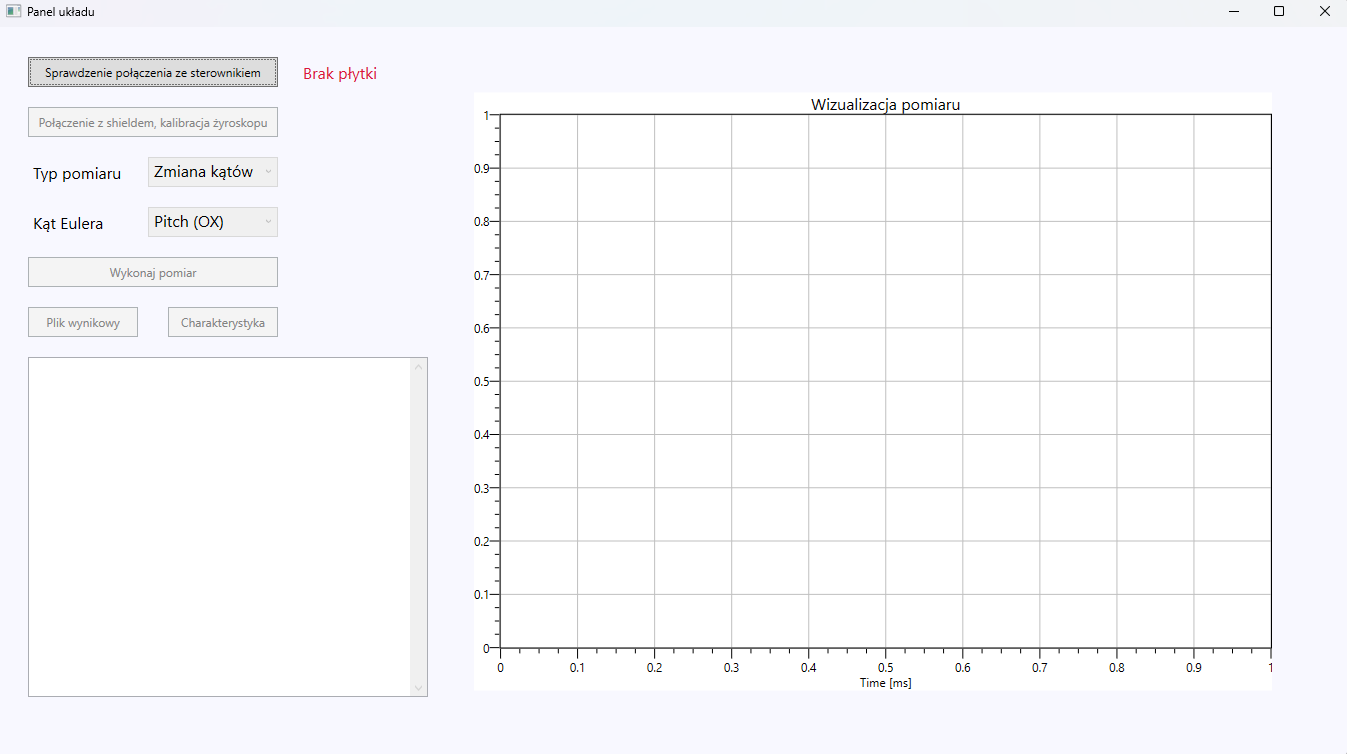
\includegraphics[width=0.48\textwidth]{pictures/app_wo.png}
    }
    \hfill
    \subfloat[Okno z płytką\label{subfig-2:w}]
    {
      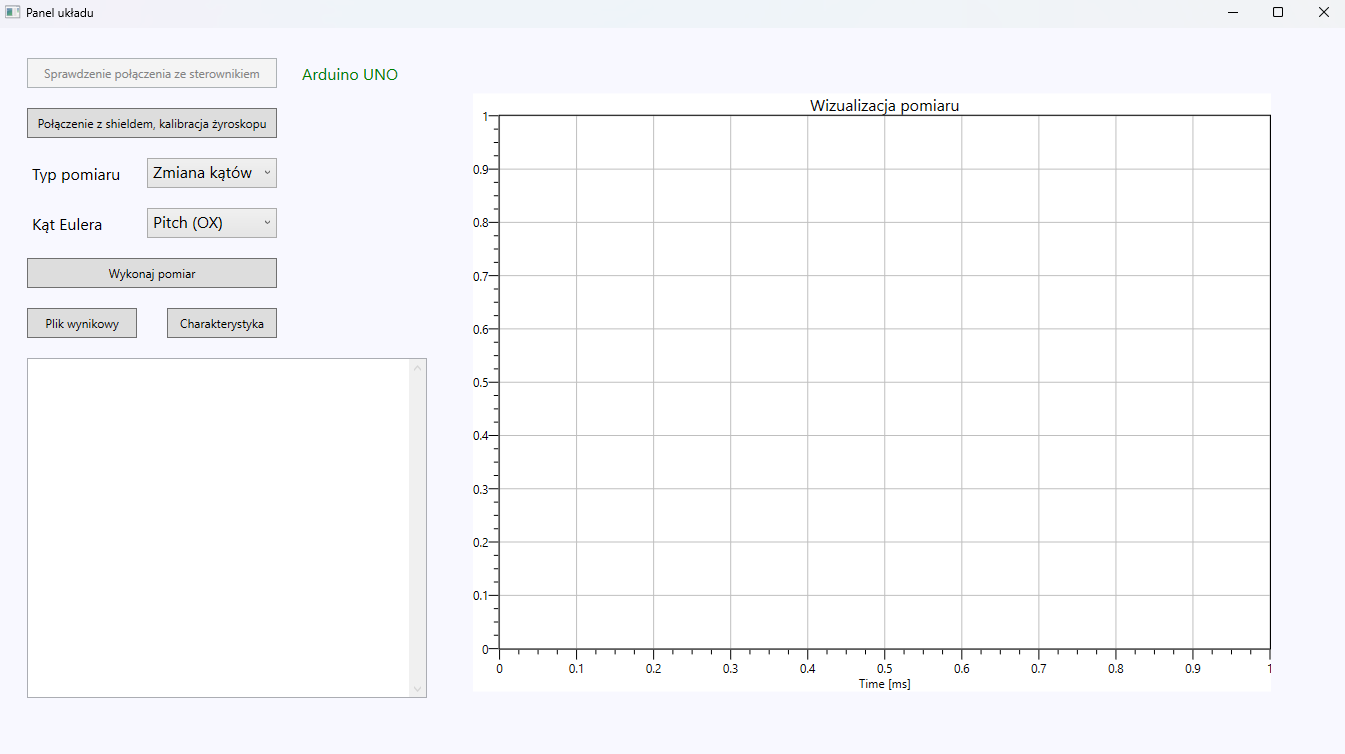
\includegraphics[width=0.48\textwidth]{pictures/app_w.png}
    }
    \caption{Okno aplikacji}
    \label{fig:app}
\end{figure}

Aplikacja pozwala na pomiar:

\begin{itemize}
    \item położenia względem wektora przyspieszenia ziemskiego względem osi OX i OY (charakterystyka przedstawia jednocześnie dane przed i po przefiltrowaniu),
    \item zmian jednego z kątów RPY (wybranego),
    \item pomiar szumów (ponownie z filtrem i bez) - położenie dla nieruchomego czujnika.
\end{itemize}

Okno aplikacji po wykonaniu pomiaru prezentuje następujące informacje (Rys. 4.2): nastawy wyboru (położenie i pitch), wartości pomiarowe w oknie tekstowym oraz wykres zależności wybranego kąta od czasu.

\begin{figure}[H]
    \centering
    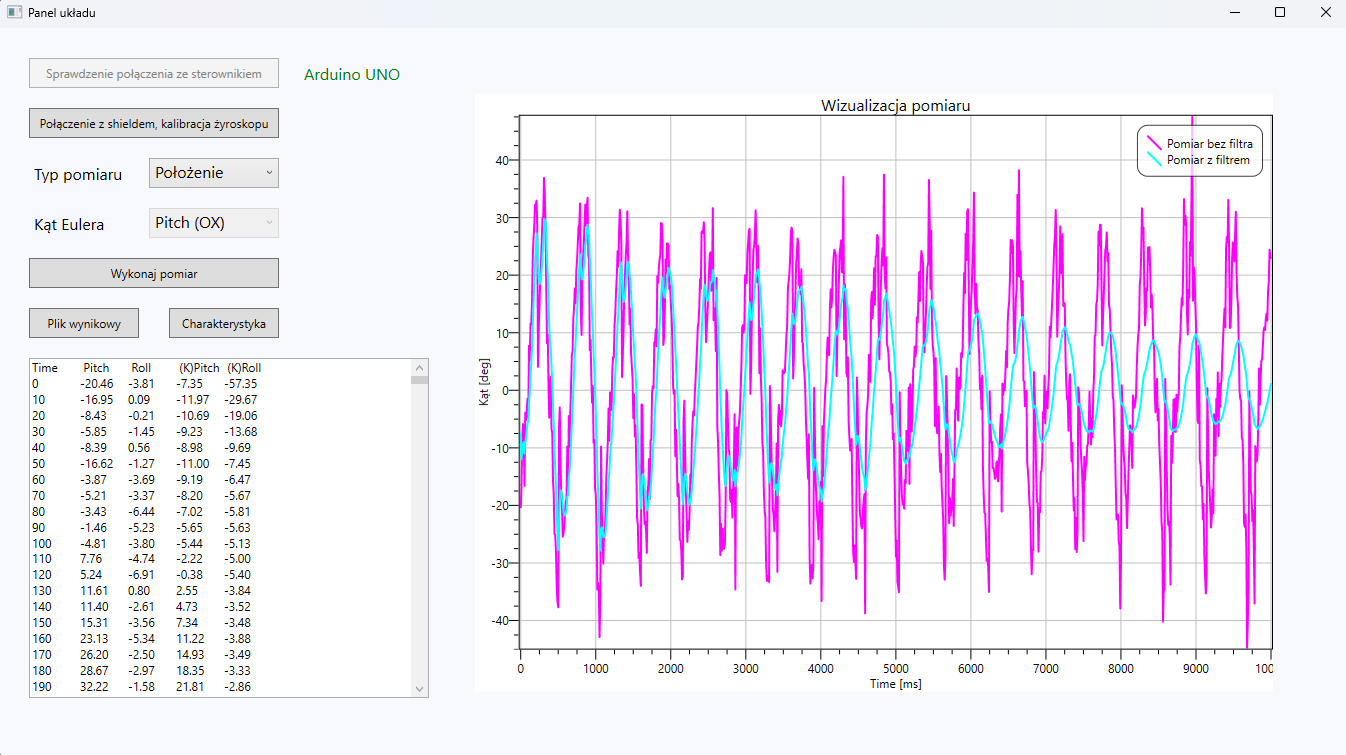
\includegraphics[width=\textwidth]{pictures/example.png}
    \caption{Przykład działania aplikacji}
    \label{fig:my_label}
\end{figure}

\subsection{Klasa aplikacji}

\lstinputlisting[caption=Metoda BtnStart\_OnClick(), language=csh, firstline=99, lastline=120]{listings/MainWindow.xaml.cs}

Listing 4.5 prezentuje główną metodę programu (odpowiadającą za obsługę przycisku \emph{Wykonaj pomiar}). Wyglądem przypomina funkcję \lstinline{void loop()}, z tą różnicą, że ta wysyła informację. Wariant dla szumu i położenia wysyła tę samą informację do płytki Arduino, ten pierwszy jednak dodatkowo zmienia jeszcze tytuł wykresu. Jako, że aplikacja w czasie rzeczywistym wyświetla pomiary w oknie tekstowym, należało wprowadzić wielowątkowość (linia 21), która umożliwia oprogramowaniu śledzenie zmian w zmiennej odbierającej dane (na bazie \cite{csh}).

Jednak zanim możliwe będzie wykonanie pomiarów, program musi upewnić się, że płytka Arduino jest dostępna. Służy do tego metoda \lstinline{BtnCheck_OnClick()}.

\lstinputlisting[caption=Metoda BtnCheck\_OnClick(), language=csh, firstline=71, lastline=93]{listings/MainWindow.xaml.cs}

Powyższy fragment kodu próbuje uruchomić połączenie szeregowe. Jeśli jest to wykonalne, kontakt zostanie nawiązany (o czym program poinformuje) i odblokowane zostaną wszystkie nastawy. W przeciwnym wypadku zostanie wystosowany komunikat o braku płytki (Rys. 4.1).

Ze względu na specyfikę kompilatora języka C\# należało opracować metodę do modyfikacji danych (listing 4.7), ponieważ ten wymusza separator dziesiętny w zależności od ustawień regionalnych systemu operacyjnego. Okazało się to o tyle problematyczne, że dane generowane przez moduł SEN0142 część ułamkową miały zapisaną po kropce, gdy w Polsce oficjalnie jest to przecinek. Metoda (dla pomiarów z filtrem) dodatkowo pomija pomiary z pierwszych $200$ ms, ze względu na wartości z filtra, które są obarczone błędem grubym.

\newpage

\lstinputlisting[caption=Metoda ModifyData(), language=csh, firstline=225, lastline=242]{listings/MainWindow.xaml.cs}

Największą i najbardziej skomplikowaną metodą jest \lstinline{BtnShow_OnClick()}. Odpowiada on w głównej mierze za rysowanie wykresów. Na poniższych listingach zostały zaprezentowane jedynie najważniejsze fragmenty kodu - ze względu na bardzo dużą ilość warunków logicznych, gdzie na każdą wariację przypadają podobne akcje, co najwyżej z innymi parametrami. Pokazano również fragmenty o unikalnym działaniu.

\lstinputlisting[caption=BtnShow\_OnClick - rozdzielanie danych), language=csh, firstline=139, lastline=140]{listings/MainWindow.xaml.cs}

Listing 4.8 prezentuje podział danych pobranych z okna tekstowego aplikacji za pomocą systemu zapytań kwerend LINQ. Na podstawie konkretnej sekwencji ucieczki (\lstinline{\n} lub \lstinline{\t}) dane są odpowiednio podzielone na dwuwymiarową tablicę.

\lstinputlisting[caption=BtnShow\_OnClick - kreślenie charakterystyki, language=csh, linerange={154-159,164-164,173-176}]{listings/MainWindow.xaml.cs}

Listing 4.9 prezentuje kolejne polecenia, które trzeba wykonać, by otrzymać charakterystykę. Wymagane jest każdorazowe wyczyszczenie siatki wykresu w celu zlikwidowania poprzednich wykresów.

\lstinputlisting[caption=BtnShow\_OnClick - zapobieganie złemu kreśleniu, language=csh, firstline=191, lastline=193]{listings/MainWindow.xaml.cs}

Jako, że położenie mierzone jest względem osi $OX$ lub $OY$, należy zabezpieczyć oprogramowanie przed potencjalną próbą wykonania analogicznej operacji dla osi $OZ$. Powyższy listing sprawia, że w przypadku takiej próby, program wyświetli komunikat z ostrzeżeniem.

Ostatnia metoda, którą użytkownik może wywołać za pomocą przycisku, jest zapisanie pomiarów do pliku tekstowego (.txt). Funkcja jednak nie tworzy katalogu, zakłada że taki już istnieje.

\lstinputlisting[caption=Metoda BtnFile\_OnClick(), language=csh, firstline=125, lastline=131]{listings/MainWindow.xaml.cs}

\section{Pomiar szumów}

W celu oceny wykonano dwa pomiary szumów - dla czujnika leżącego i stojącego. Otrzymano następujące charakterystyki:

\begin{figure}[H]
    \subfloat[Szum dla $\theta$\label{subfig-3:theta_sit}]
    {
      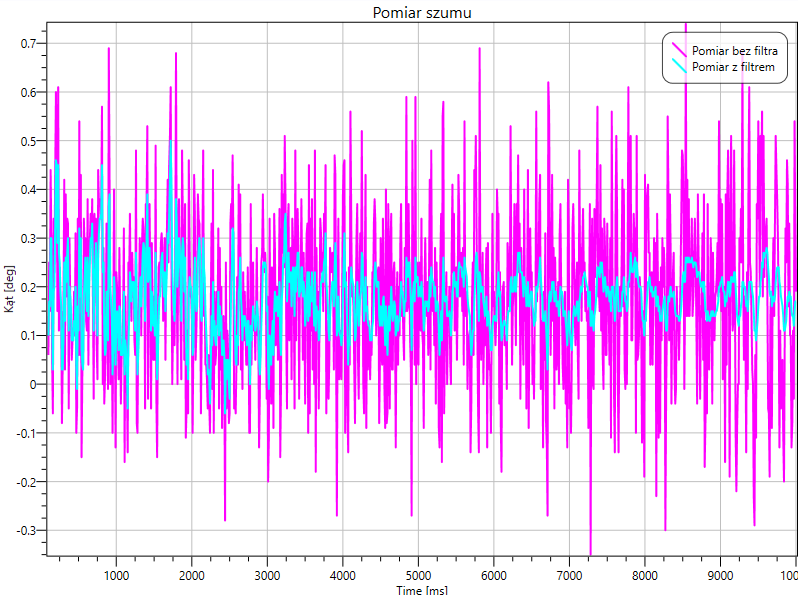
\includegraphics[width=0.48\textwidth]{pictures/theta_sit.png}
    }
    \hfill
    \subfloat[Szum dla $\phi$\label{subfig-4:phi_sit}]
    {
      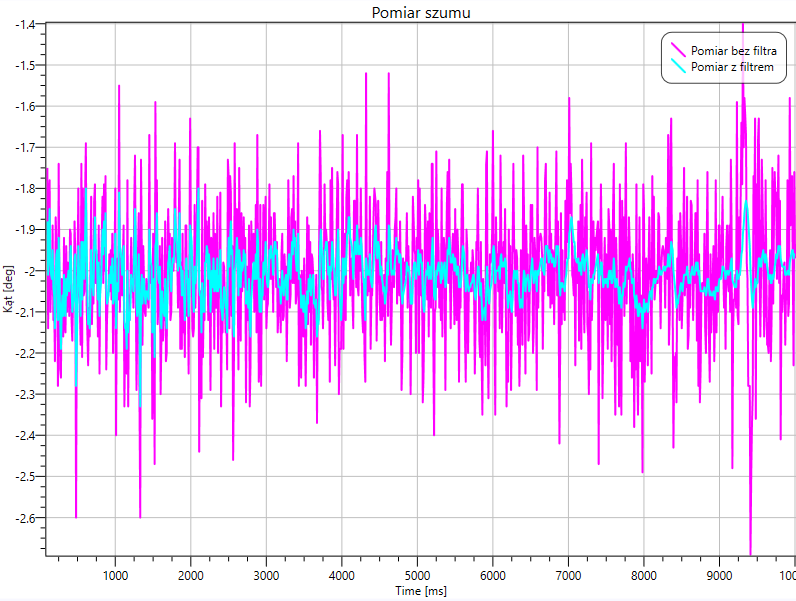
\includegraphics[width=0.48\textwidth]{pictures/phi_sit.png}
    }
    \hfill
    \subfloat[Szum dla $\theta$\label{subfig-5:theta_stand}]
    {
      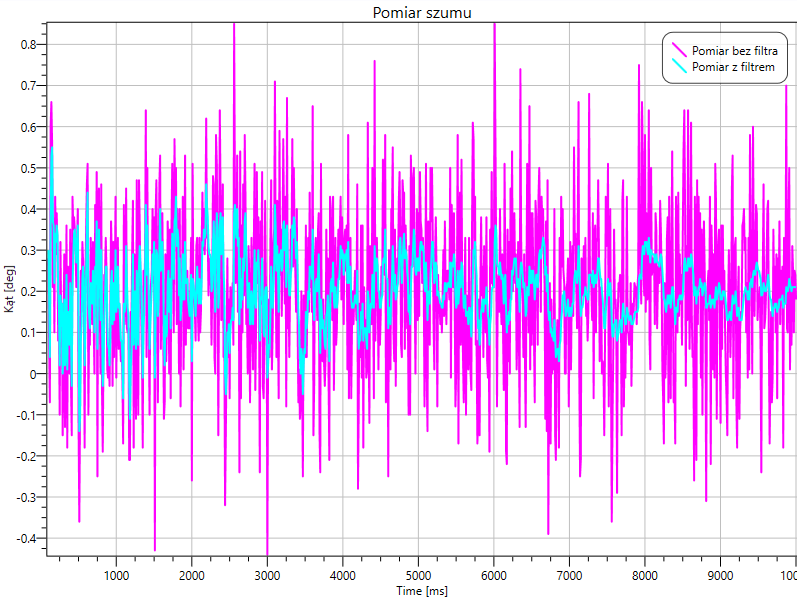
\includegraphics[width=0.48\textwidth]{pictures/theta_stand.png}
    }
    \hfill
    \subfloat[Szum dla $\phi$\label{subfig-6:tphi_stand}]
    {
      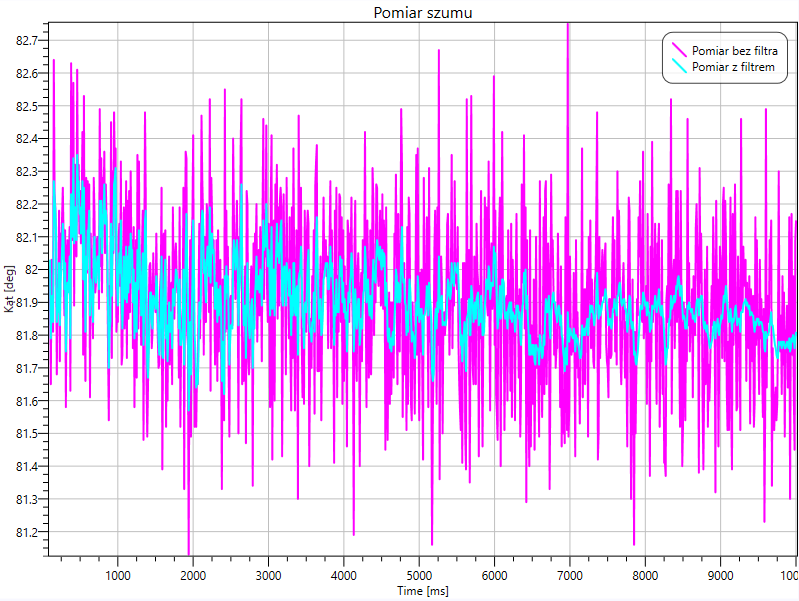
\includegraphics[width=0.48\textwidth]{pictures/phi_stand.png}
    }
    \caption{Charakterystyki czujnika: leżącego ((a) i (b)) i stojącego ((c) i (d))}
    \label{fig:szum_sit}
\end{figure}

Widać, że podane szumy w każdym z przypadków wprowadzają niepewność pomiarową wynoszącą $1^{o}$. Filtr zmniejsza ją do poziomu $0.5^{o}$. Jednak by ten zaczął poprawnie działać potrzebne jest kilkadziesiąt próbek by estymacja osiągała sensowne wartości.

\section{Pomiary laboratoryjne}

Moduł SEN0142 został zamocowany do elementu obrotowego silnika za pomocą kleju \emph{Kropelka}. Został on wytypowany na podstawie tego, że wiąże materiały na sztywno, tak więc czujnik nie będzie ciągnięty przez powierzchnię, na której się znajduje, a raczej stworzy z nią integralną całość. W pierwszej kolejności po przymocowaniu czujnika wykreślono jego szum:

\begin{figure}[H]
    \subfloat[Szum dla $\theta$\label{moc1}]
    {
      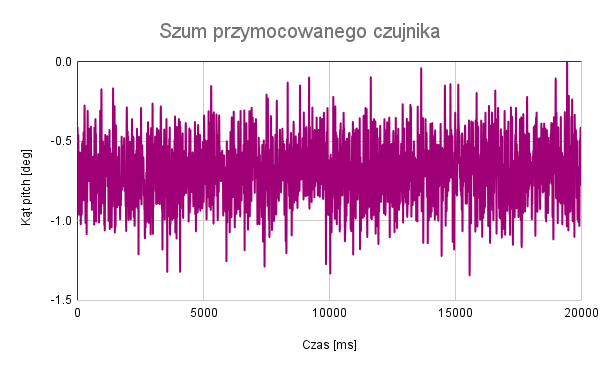
\includegraphics[width=0.48\textwidth]{pictures/szum_mocowanko.png}
    }
    \hfill
    \subfloat[Szum dla $\phi$\label{moc2}]
    {
      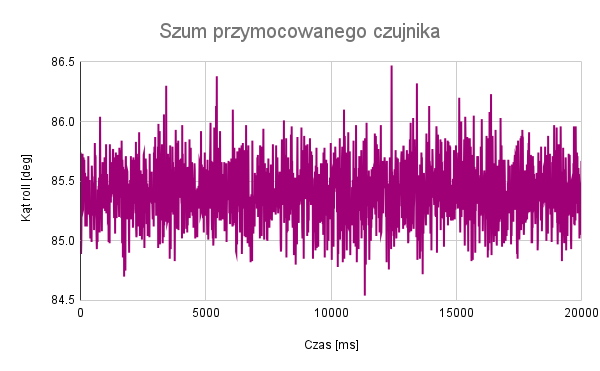
\includegraphics[width=0.48\textwidth]{pictures/szum_mocowanko_2.png}
    }
    \caption{Wykresy dla przymocowanego czujnika}
    \label{fig:szumu_szumu}
\end{figure}

Uśredniając pomiary wykorzystane do wykresów otrzymano wartości początkowe (wraz z ich odchyleniami standardowymi) w jakich ustawiony jest czujnik. Wyniosły one:

\begin{itemize}
    \item Kąt pitch $\theta = -0.69 \pm 0.19$ [deg]
    \item Kąt roll $\phi = 85.41 \pm 0.25$ [deg]
\end{itemize}

Widać, że wartości nie wynoszą idealnie $0^{o}$ i $90^{o}$. Biorąc pod uwagę, że sam LCT znajduje się w fazie prototypowej, należy uwzględnić błąd wynikający z ręcznego składania urządzenia (np. fakt, że samo zwierciadło nie jest idealnie wycentrowane).

Po włączeniu symulacji na tomografie i załączeniu pomiaru położenia w aplikacji, czujnik po kilku pomiarach zamilkł. W przypadku pomiaru zmiany kątów żyroskopem nie otrzymano żadnej odpowiedzi. 

\begin{table}[H]
    \centering
    \caption{Otrzymane wyniki podczas ruchu zwierciadła}
    \begin{tabular}{l|cccc}
        \toprule
            Czas [ms]  &     0 &    10 &     20 &     30 \\
            Pitch [deg] & 64.75 & 62.86 & -46.87 & -54.72 \\
            Roll [deg] & 24.61 & 24.63 &  25.09 &  23.43 \\
        \bottomrule
    \end{tabular}
    \label{tab:ruch_false}
\end{table}

\newpage

Po wykreśleniu dane przedstawiły się następująco:

\begin{figure}[H]
    \centering
    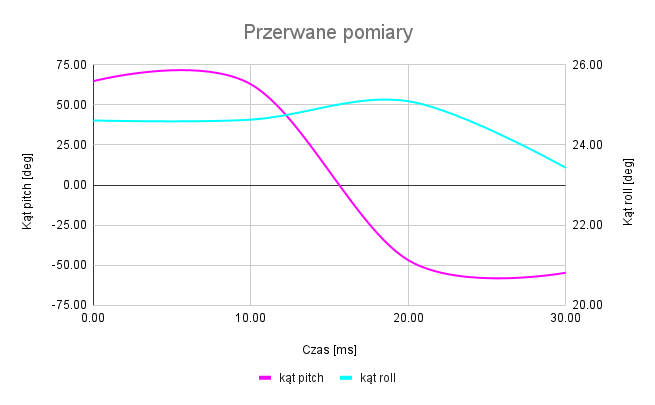
\includegraphics[width=\textwidth]{pictures/false.png}
    \caption{Nieukończone pomiary}
    \label{fig:false}
\end{figure}

Na charakterystyce kąta pitch widać, zapoczątkowanie ruchu okresowego, jednakże nic więcej nie da się z owej wizualizacji wywnioskować.

Potencjalnym źródłem błędów mogą być asymetryczne działanie momentów bezwładności wprowadzone przez przewody podłączone do czujnika. Przewody zostały ze sobą sklejone oraz usztywnione w odpowiednich miejscach, przyjęto więc wzór na moment bezwładności prętu o długości $l$ nachylonego do osi obrotu pod kątem $\alpha$.

\begin{equation}
    I = \frac{1}{3}ml^{2}\sin^{2}{\alpha}
\end{equation}

W celu wyznaczenia niepewności wykorzystano metodę różniczki zupełnej:

\begin{equation}
    \delta I = \Bigg|\frac{\partial I}{\partial m}\Bigg| \delta m + \Bigg|\frac{\partial I}{\partial l}\Bigg| \delta l + \Bigg|\frac{\partial I}{\partial \alpha}\Bigg| \delta \alpha
\end{equation}

Dane:
\begin{itemize}
    \item $m = 18 \pm 1$ [g],
    \item $l = 45.0 \pm 0.1$ [cm],
    \item $\alpha = 60^{o} \pm 5^{o}$
\end{itemize}

Moment bezwładności otrzymany wraz z niepewnością wyniósł:

$$
I = \frac{1}{3} \cdot 18 \cdot 45^{2} \cdot \sin^{2}{60} = 0.911 \pm 0.005 \; [kg \cdot m^{2}]
$$

Widać, że moment ten występuje, może więc on bezpośrednio zaburzać ruch masy w akcelerometrze, przez co czujnik przestaje odczytywać dane. Dodatkowo, przez ręczne zamontowanie elementów (zwierciadło, czujnik) elementy te nie są umieszczone idealnie symetrycznie, co w efekcie wprowadza asymetrię do rozkładu momentów bezwładności.